% This is samplepaper.tex, a sample chapter demonstrating the
% LLNCS macro package for Springer Computer Science proceedings;
% Version 2.20 of 2017/10/04
%
\documentclass[tikz, runningheads]{llncs}
%
\usepackage{graphicx}
\usepackage[linguistics]{forest}
\usepackage{adjustbox}
\usepackage{float}
% Used for displaying a sample figure. If possible, figure files should
% be included in EPS format.
%
% If you use the hyperref package, please uncomment the following line
% to display URLs in blue roman font according to Springer's eBook style:
% \renewcommand\UrlFont{\color{blue}\rmfamily}


\forestset{
    sn edges/.style={for tree={parent anchor=south, child anchor=north}},
    red subtree/.style={for tree={text=red},for descendants={edge=red}},
    black subtree/.style={for tree={text=black},for descendants={edge=black}}}

%\setlength{\belowcaptionskip}{-10pt}
%\setlength\intextsep{2pt}

\begin{document}
%
\title{Evolve Bagging Ensembles with Genetic Programming}
%
%\titlerunning{Abbreviated paper title}
% If the paper title is too long for the running head, you can set
% an abbreviated paper title here
%
\author{Korbinian Federholzner}
%
\authorrunning{Federholzner K.}

% First names are abbreviated in the running head.
% If there are more than two authors, 'et al.' is used.
%
\institute{Ludwig Maximilian University of Munich, Munich 80539, Germany
\email{K.Federholzner@campus.lmu.de}}

%
\maketitle              % typeset the header of the contribution
%
\begin{abstract}
\textit{Bagging} is a common method in Machine Learning to get more accuracy for predictors. Applied to \textit{Genetic Programming (GP)} 
this can have a big advantage, in getting better results. There are multiple implementations of such algorithms that focus on getting better performance on 
\textit{GP} with \textit{Bagging}. Most of those algorithms tend to be complex in implementation and fast or simple and slow.
The algorithm presented in this paper called \textit{Simple Simultaneous Ensemble Genetic Programming (2SEGP)} tries to extend classic \textit{GP} with \textit{bagging} only by a few features to 
be simple as possible but also provides a similar speed to the more complex implementations. 

\keywords{Genetic programming \and ensemble learning \and machine learning \and bagging \and evolutionary algorithms}
\end{abstract}
%
%
%
\section{Introduction}
\textit{GP} algorithms are typically used to approximate solutions to NP-Hard Problems as well as 
other optimization problems that normally would be too computationally expensive. 
Even though those solutions are often good enough they can never be viewed as optimal due to the random 
nature of \textit{GP}. In Machine Learning (ML) a technique called \textit{bagging} is used to get a better approximation of the 
resulting predictors. Some \textit{GP} algorithms try to use \textit{bagging} because of that reason. Using \textit{bagging} without modifying 
the \textit{GP} algorithm will increase the run time by a lot and thus a lot of complex \textit{GP} algorithms have emerged that 
try to tackle this issue. One algorithm \textit{2SEGP}, the algorithm discussed in this paper, does this by also trying to not have the 
complexity of implementation that would normally come from those modifications. This paper starts in section \ref{sectionGP} 
by explaining the basics on which most \textit{GP} algorithms are built. Followed by section \ref{sectionBagging} in which 
the basics of \textit{bagging} are shown. Section \ref{section2SEGP} than shows how \textit{2SEGP} unites the basics explained 
in the previous sections to a new algorithm. Lastly, the paper is finished off with a Conclusion in section 
\ref{sectionConclustion}.

\section{Genetic Programming}
\label{sectionGP}
The Darwinian theory by Charles Darwin is the theory, that individuals of a species of organisms survive natural selection
and develop with the help of reproduction and inheritance \cite{darwin}. A class of algorithms, 
in \textit{computational intelligence}, called the \textit{Evolutionary Algorithms}, 
try to model this theory. One of those algorithms, \textit{Genetic Programming (GP)} does this with the help of 
syntax trees. The nodes of a syntax tree are represented by arithmetic operations 
(+, -, *, /, min, ...) called functions, while the leaves are variables and constants (x, a, 1, 2, ...) called terminals.
Traversing the tree is done bottom-up from a leaf to the root node. 
Figure \ref{Tree1} shows a syntax tree that is constructed from the formula: $(\frac{y}{2.33}) * \log(x) + \max((x + 2), x)$


\begin{figure}[h]
	\centering
	\scalebox{1}{
	\begin{forest}
		[+
			[*
				[/
					[y]
					[2.33]
				]
				[log
					[x]	
				]
			]
			[max
				[+
					[x]
					[2]
				]
				[x]
			]
		]
	\end{forest}
	}
	\caption{Syntax tree of a \textit{GP} algorithm with the formula: $(\frac{y}{2.33}) *  \log(x) + \max((x + 2), x)$} \label{Tree1}
\end{figure}



\textit{GP} algorithms generally have the same structure, as shown in figure \ref{OverviewImage}. 
They start with an initial population of randomly created subtrees.
Those individuals get their fitness value calculated. Followed by a selection, weighted by the fitness values, in which the parents
are chosen. In the crossover step, the parents create new offspring until the new population has the same size of individuals as the
old population. The newly created children each have a small chance to be mutated. This procedure gets repeated until the
termination criteria is met. This can be for example either a fixed maximum of iterations or iteration until the newly created children 
do not change anymore.

\begin{figure}
	\centering
	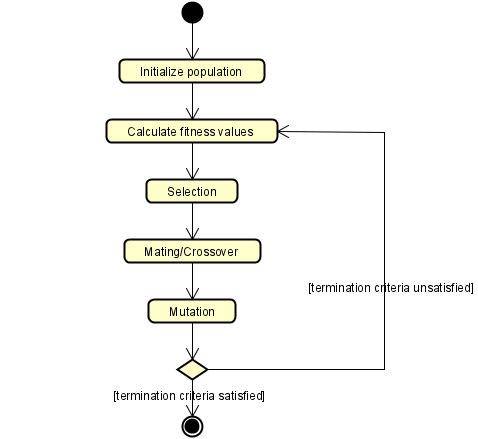
\includegraphics[scale=0.7]{Images/OverviewDiagram.PNG}
	\caption{An overview of the general procedure of a \textit{GP} algorithm} \label{OverviewImage}
\end{figure}

\subsection{Initial Population}
As a starting point for a given number of individuals in the population, there are N random trees generated. 
From a given set of functions and terminals, each node of a tree gets assigned a random function and each leaf 
a random terminal. There are multiple ways of filling up the tree, such as the \textit{grow}, \textit{full} and 
\textit{ramped half-and-half} methods. Essentially a tree gets filled until a specified depth. 
In the \textit{full} method, all leaves have the same depth. The \textit{grow} method stops when it hits the depth limit 
and then fills its leaves \cite{FieldGuideToGP}. This results in a tree, that has terminals on different depth levels.\textit{Ramped half-and-half} initializes half the population with the \textit{full} method 
and the other half with the \textit{grow} method \cite{Koza}. Figure \ref{fullAndGrow} shows two trees 
generated from \textit{full} and \textit{grow}.

\begin{figure}[h]
	\centering
	\begin{adjustbox}{valign=t}
		\begin{forest}
			[*
				[-
					[1]
					[y]
				]	
				[+
					[x]
					[1]
				]
			]
		\end{forest}
	\end{adjustbox}\qquad
	\begin{adjustbox}{valign=t}
		\begin{forest}
			[+
				[-
					[x]
					[5]
				]
				[y]	
			]
		\end{forest}
	\end{adjustbox}
	\caption{The left syntax tree shows a tree generated with the \textit{full} method and the right tree shows a tree
	generated with the \textit{grow} method} \label{fullAndGrow}
\end{figure}
 

\subsection{Fitness}
Similar to the phrase "survival of the fittest" from Darwin's evolutionary theory, the best individuals in 
the population of a \textit{GP} algorithm should have the highest probability to survive and create new offspring. 
The performance of an individual is measured with a fitness function. 
The closer the value of a fitness function is to the desired value the better the individual. 
The fittest individuals have the highest chance to mate and create new children for the next generation.  
Fitness functions often get measured with \textit{mean squared error (MSE)} or the \textit{mean absolute error (MAE)}. 

\subsection{Selection}
For the creation of a new generation, a selection process is needed. 
In this process, the parents are getting chosen to favor the individuals with the best fitness values.
Choosing the $\frac{1}{p}$ fittest individuals is called \textit{truncation selection}.
The advantage of \textit{truncation selection} is that it is very easy to implement and very efficient. 
But choosing only the fittest individuals is not always the best idea, since it might come with a loss of diversity.
This is because the children of the fittest individuals will most likely be the fittest individuals
in the next generation. Since the fittest will also have most children, this will lead to a population where 
almost all individuals have some sort of heritage from the same parents and thus converge to 
a single individual. In \textit{tournament selection}, $n$
random individuals from the population are chosen, which then get compared to each other. The fittest of them 
are chosen to be parents. Two or more tournament-winning individuals are then used for the generation of a new child.  
This procedure is repeated until there have been enough parents chosen to create a new generation has the 
same size as the old population \cite{Selection}.
\textit{Tournament selection} on the other hand guarantees more diversity because individuals are chosen at random. 
There could be a scenario where the best individual never gets chosen for a tournament and thus never gets to
create a child. 

\subsection{Crossover}
In Crossover two or more individuals that have survived the selection produce offspring. The goal of this step is to 
create a new population of children of the same size as the previous one. In \textit{GP} the most common variant is 
\textit{subtree crossover}. First, a node, called the crossover point is selected for each parent, then everything 
above, up to the root node, is removed in the first parent. For the second parent, the crossover point and everything below it  
is removed. Both then merge at crossover points, as illustrated in Figure \ref{mating}. All of those 
operations are done on a copy of the parents to not lose the parents because they could be needed for the creation 
of more offspring. The crossover operation can be set to a certain probability (commonly 90\%), which means it 
is not applied every time. In that case, either \textit{mutation} or \textit{reproduction} is used. 
\textit{Reproduction} simply copies the fitter parent to the next generation. 
% crossover might only use leaves (small alteration) to counter this 90% functions used and 10% leaves 

\begin{figure}[h]
	\centering
	\begin{adjustbox}{valign=t}
		\begin{forest}
			[$*$
				[-
					[1]
					[y]
				]	
				[\textcolor{blue}{+}, red subtree
					[x]
					[1]
				]
			]
		\end{forest}
	\end{adjustbox}\qquad
	\begin{adjustbox}{valign=t}
		\begin{forest}
			[+, red subtree
				[\textcolor{blue}{$*$}, black subtree
					[x]
					[5]
				]
				[y]	
			]
		\end{forest}
	\end{adjustbox}\qquad
	\begin{adjustbox}{valign=t}
		\begin{forest}
			[+
				[+
					[x]
					[1]
				]
				[y]	
			]
		\end{forest}
	\end{adjustbox}
	\caption{The blue functions mark the crossover points and the red marked subtrees are the subtrees used for the 
	offspring. The third tree shows the resulting child for the next generation} \label{mating}
\end{figure}

\subsection{Mutation}
Since the initial population is generated randomly, some possible subtree combinations might be missing. 
To combat this, \textit{mutation} is used. The most common mutation variant called is
\textit{headless chicken crossover} \cite{headlessChicken}. It selects a random node of the tree and substitutes
it with a new randomly created subtree. Another form of mutation is \textit{point mutation} \cite{pointMutation}. In this form, 
a random node gets selected, but instead of replacing the whole subtree, only the node itself gets changed 
to a new primitive. Generally, the \textit{mutation rate} is very small, most of the time around 1\%. Figure \ref{mutation}
takes the child produced in figure \ref{mating} and shows an example of what applying those mutations could look like.

\begin{figure}[htbp]
	\centering
	\begin{adjustbox}{valign=t}
		\begin{forest}
			[+
				[+
					[x]
					[1]
				]
				[y]	
			]
		\end{forest}
	\end{adjustbox}\qquad
	\begin{adjustbox}{valign=t}
		\begin{forest}
			[/, red subtree
				[1.44]
				[y]
			]
		\end{forest}
	\end{adjustbox}\qquad
	\begin{adjustbox}{valign=t}
		\begin{forest}
			[+
				[/, red subtree
					[1.44]
					[y]
				]	
				[y]
			]
		\end{forest}
	\end{adjustbox}\qquad
	\begin{adjustbox}{valign=t}
		\begin{forest}
			[\textcolor{blue}{*}
				[+
					[x]
					[1]
				]
				[y]	
			]
		\end{forest}
	\end{adjustbox}
	\caption{The first tree is the child from figure \ref{mating}, the second red tree is the random subtree which was produced 
	using \textit{headless chicken crossover}, which then gets applied to result in tree number three. On the last tree, 
	\textit{point} mutation was applied on the root node.} \label{mutation}
\end{figure}

\section{Bagging}
\label{sectionBagging}
\textit{Bagging}, also known as \textit{\textbf{b}ootstrap \textbf{agg}regat\textbf{ing}}, is a method for gaining 
more accuracy through the aggregation of multiple predictors. To get $\beta$ predictors, 
the training set $T$ has to be sampled with 
replacement, to get multiple realizations $T_1, T_2, ..., T_\beta$, also called bootstrap samples, of the original training set $T$. 
The predictors trained by those training sets, have to be aggregated, traditionally with a majority voting 
for classification or averaging for regression \cite{bagging}. 

\section{Simple Simultaneous Ensemble Genetic Programming (2SEGP)}
\label{section2SEGP}
There are many algorithms that combine \textit{Bagging} and \textit{GP}, those can be categorized into
\textit{Simple Independent Ensemble Learning Approaches(SIEL)} and \textit{Complex Simultaneous Ensemble
Learning Algorithms (CSEL)}. \textit{SIEL}-applications, are very simple, they execute \textit{GP} on each of the 
bootstrapped training sets and then aggregate all estimators to a single estimation. This makes 
them very simple to implement, but inefficient.
\textit{CSEL}-algorithms, on the other hand, are very complex and efficient. They try to evaluate an ensemble in one go.
\textit{2SEGP} is an algorithm that tries to have the simplicity of a \textit{SIEL}-application, while being 
comparable in performance to a \textit{CSEL}-Algorithm. To accomplish this the \textit{2SEGP} changes two classical
aspects of a generic \textit{SIEL}-application, the individual selection and the fitness function.
Other than that, the initialization uses \textit{Ramped half-and-half}, but it increments the depth of the trees, to get 
even more variation. The calculation of the fitness value uses the \textit{MSE}, on which \textit{linear scaling} is applied \cite{LinearScaling}. 
Mating is done with \textit{subtree crossover} and mutation with \textit{headless chicken crossover} \cite{GPoriginal}. 

\subsection{Individual Selection}
The \textit{2SEGP} algorithm modifies the selection of \textit{bagging} slightly. Each individual gets evaluated uniformly 
across all bootstrap samples, which means it doesn't have a single fitness value, it has $\beta$ of them. 
Each individual, disregarding fitness, creates a child with either the \textit{mutation} or \textit{subtree crossover} operations applied. 
In the case of \textit{subtree crossover}, another random individual is selected. The reason for not taking 
fitness into account when producing children is, that most of the time the top-ranked individuals 
are very similar to each other. This leads to a drop-off in the variation of individuals.
Instead, each child gets calculated a new fitness value. Together with all parents and children, the top $\frac{n_{pop}}{\beta}$ 
individuals, ranked by fitness, for each bootstrap sample $T_1, T_2, ..., T_\beta$, get chosen. This has a similar effect as 
just using the best parents for reproduction since bad individuals are not selected for the next generation. 

%graphic here%

\subsection{Changes to Fitness-Evaluation}
Since each individual gets evaluated over all bootstrap samples $T_1, T_2, ..., T_\beta$ and the size of each 
sample is the same as the original sample $T$, this would lead to a high cost of computation. \textit{2SEGP} utilizes 
the property that each sample is derived from the original sample $T$. Instead of computing a value for each 
$T_1, T_2, ..., T_\beta$, the value of an individual gets just computed once for $T$. A separate collection of 
indices is held for each bootstrap sample $S_1, S_2, ..., S_\beta$. Each $S_j$ contains $n$ indices that 
correspond with an index from the original sample $T$. Rather than recomputing each sample, the value computed for 
the original $T$ corresponding to the index gets used. This results in the computational complexity of 
$O(ln) + O(n\beta) + O(n\beta) = O(n(l + \beta))$. where $l$ is the operation cost for traversing the whole 
tree and $n$ is the number of samples of the training set. In the case of an \textit{SIEL}-algorithm, this complexity 
would be $O(nl\beta)$, since every individual would have to be trained $n$ times on every bootstrap sample 
$T_1, T_2, ..., T_\beta$.


\subsection{Linear Scaling of fitness}
Scaling the fitness function can have huge benefits since it helps not run into dead ends, where the 
most dominant individuals of a population all converge into one individual, thus losing diversity.
If done right Scaling will increase the performance of a \textit{GP} algorithm. There are a lot of 
different ways to scale the fitness function, \textit{2SEGP} uses Linear Scaling. 
This reduces the \textit{MSE} of a syntax tree, by applying an optimal linear transformation to the outputs. 
It's computed by applying the slope and the intercept and then scaling the \textit{MSE} with it:

\begin{equation}
	a = \overline{y} - b\overline{o}
\end{equation}
\begin{equation}
	b = \frac{\sum_{i = 1}^{n} (y_i - \overline{y})(o_i - \overline{o})}{\sum_{i = 1}^{n} (o_i - \overline{o})^2}
\end{equation}
\begin{equation}
	MSE^{a,b}(y, o) = \frac{1}{n} \sum_{i = 1}^{n} (y_i -(a + bo_i))^2
\end{equation}

Where $y$ contains the labels, $o$ the outputs of the syntax trees after the evaluation, $n$ the size of the data set and $a, b$
being both of the coefficients. $\overline{o}$ and $\overline{y}$ represent the mean of the respective variables.
This doesn't increase the complexity by a lot, but increases the performance, for a lot of problems. 

%graphic here%

\subsection{Example run}
To show a very simple example run of \textit{2SEGP} the code from \cite{Github2SEGP} is used. For the parameters, 
a population size of $n_{pop} = 4$ and an ensemble size of $\beta = 2$ are chosen. 
As data set $T$ the Boston housing prices are used, which has $|T| = 500$ samples and $d = 13$ features. This results in a function set 
of $\{+, -, *, /\}$ and a terminal set of $\{erc, x_1, x_2, ..., x_{13}\}$. $erc$ is
Ephemeral Random Constant (ERC) as proposed by Koza \cite{Koza} and describes a random numerical constant that is 
inserted in case it gets chosen. Each of the 13 features from the data set, gets a
variable ($x_1, x_2, ..., x_{13}$). Since trees get chosen by \textit{Ramped half-and-half} and depth starts at 2, with increments until a threshold, the 
random trees generated will look like the trees in Figure \ref{exampleInitialPop}.

\begin{figure}[htbp]
	\centering
	\begin{adjustbox}{valign=t}
		\scalebox{0.7}{
		\begin{forest}
			[-
				[/
					[$x_4$]
					[$x_5$]
				]	
				[-
					[$x_9$]
					[$x_8$]
				]
			]
		\end{forest}
		}
	\end{adjustbox}\qquad
	\begin{adjustbox}{valign=t}
		\scalebox{0.6}{
		\begin{forest}
			[-
				[-
					[+
						[$x_6$]
						[$-2.438$]
					]
					[+
						[$x_9$]
						[$x_8$]
					]
				]
				[/
					[*
						[$x_{11}$]
						[$x_8$]
					]
					[*
						[$x_8$]
						[$x_1$]
					]
				]	
			]
		\end{forest}
		}
	\end{adjustbox}\qquad
	\begin{adjustbox}{valign=t}
		\scalebox{0.7}{
		\begin{forest}
			[/
				[+
					[$x_{10}$]
					[$x_8$]
				]
				[$x_7$]
			]
		\end{forest}
		}
	\end{adjustbox}\qquad
	\begin{adjustbox}{valign=t}
		\scalebox{0.5}{
		\begin{forest}
			[+
				[/
					[-
						[$x_{12}$]
						[$x_{10}$]
					]
					[$x_12$]
				]
				[/
					[$3.866$]
					[$x_6$]
				]	
			]
		\end{forest}
		}
	\end{adjustbox}
	\caption{In the initial population, the top two trees are created by \textit{full} and the bottom two by 
	\textit{grow}} \label{exampleInitialPop}
\end{figure}

For reproduction, all of the created trees will produce the children with the help of \textit{subtree crossover}
and \textit{mutation}. For this example, both the probability of \textit{mutation} and \textit{subtree crossover} is set 
to 50\%. Note that this is an example and a lower \textit{mutation} rate could be better. Because of the selection process, all parents get a
chance to be included in the next generation anyways, \textit{reproduction} is not included at all.
Figure \ref{exampleChildren} shows all children that got generated.

\begin{figure}[htbp]
	\centering
	\begin{adjustbox}{valign=t}
		\scalebox{0.8}{
		\begin{forest}
			[-
				[/
					[$x_4$]
					[$x_5$]
				]	
				[-
					[$x_3$]
					[$x_8$]
				]
			]
		\end{forest}
		}
	\end{adjustbox}\qquad
	\begin{adjustbox}{valign=t}
		\scalebox{0.5}{
		\begin{forest}
			[/
				[+
					[$x_{10}$]
					[/
						[+
							[$x_{10}$]
							[$x_8$]
						]
						[$*$
							[$x_7$]
							[$x_2$]
						]
					]
				]
				[$x_7$]
			]
		\end{forest}
		}
	\end{adjustbox}\qquad
	\begin{adjustbox}{valign=t}
		\scalebox{0.6}{
		\begin{forest}
			[+
				[/
					[-
						[$x_{12}$]
						[$x_{10}$]
					]
					[$x_{12}$]
				]
				[/
					[$3.866$]
					[-
						[$x_1$]
						[$x_{12}$]
					]
				]	
			]
		\end{forest}
		}
	\end{adjustbox}\qquad
	\begin{adjustbox}{valign=t}
		\scalebox{1}{
		\begin{forest}
			[$x_4$]
		\end{forest}
		}
	\end{adjustbox}
	\caption{For the children created from the initial population, the tree with only root node $x_4$ got selected for 
	\textit{mutation} and got substituted by only one terminal} \label{exampleChildren}
\end{figure}

Each child and parent get their fitness value calculated, one for every value in the samples of $T_1$ and $T_2$. The top $\frac{n_{pop}}{\beta}$
individuals for each sample are chosen to be in the next population. Figure \ref{evalImage} shows the individual selection.
\begin{figure}[h]
	\centering
	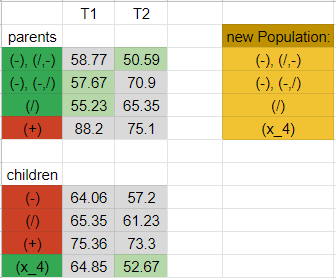
\includegraphics[scale=0.5]{Images/fitnessEval.PNG}
	\caption{The fitness evaluation of the population. Green individuals are included in the next population, 
	the other red ones are getting discarded} \label{evalImage}
\end{figure}

After the new population is formed, the \textit{2SEGP} algorithm, repeats from calculating fitness again. 
This gets repeated until a certain time is elapsed, or a specified number of populations are created.
The resulting individuals are the $\beta$ elites, the best of each sample $T_1, T_2, ... T_{\beta}$.
A majority vote between them will determine the final result for given inputs. 
After 30 generations, in the example case, the resulting elites both have the same structure.
Figure \ref{theElite}, shows the resulting elites, with both having a fitness value of 30.315 for 
$T_1$ and 29.998 for $T_2$. 

\begin{figure}[htbp]
	\centering
	\begin{adjustbox}{valign=t}
		\scalebox{0.75}{
		\begin{forest}
			[+
				[*
					[/
						[+
							[-
								[$x_3$]
								[$x_1$]
							]
							[*
								[$x_5$]
								[$-4.1$]
							]
						]
						[$x_2$]
					]
					[+
						[-
							[$x_5$]
							[$x_{11}$]
						]
						[$x_8$]
					]
				]	
				[/
					[$x_3$]
					[-
						[$x_4$]
						[$x_{12}$]
					]
				]
			]
		\end{forest}
		}
	\end{adjustbox}\qquad
	\begin{adjustbox}{valign=t}
		\scalebox{0.57}{
		\begin{forest}
			[+
				[*
					[/
						[+
							[-
								[$x_3$]
								[$x_1$]
							]
							[*
								[$x_5$]
								[$-4.1$]
							]
						]
						[$x_2$]
					]
					[+
						[-
							[$x_5$]
							[$x_{11}$]
						]
						[$x_8$]
					]
				]	
				[/
					[$x_3$]
					[-
						[$x_4$]
						[$x_{12}$]
					]
				]
			]
		\end{forest}
		}
	\end{adjustbox}
	\caption{The resulting elites, in this example the last two individuals are exactly the same} \label{theElite}
\end{figure}


\subsection{Comparision with state-of-the-art algorithms}
The paper \cite{GPoriginal} compares \textit{2SEGP} to other state-of-the-art algorithms, by comparing them on accuracy. 
On both the tasks of classification and regression, the represented algorithms that are considered some of the leading ones 
for those tasks are chosen. The algorithms for classification are:
\begin{itemize}
	\item Diverse Niching Genetic Programming (DNGP) \cite{DNGP}
	\item Ensemble GP with weighted voting (eGPw) \cite{EnsembleGeneticProgramming}
	\item Multidimensional Multiclass GP with Multidimensional Populations (M3GP) \cite{EnsembleGeneticProgramming}
	\item Classic Genetic Programming (cGP)
\end{itemize}
And for the regression task:
\begin{itemize}
	\item Diverse Niching Genetic Programming (DNGP) \cite{DNGP}
	\item Spatial Structure with Bootstrapped Elitism (SS+BE) \cite{SS+BE}
	\item Gene-pool Optimal Mixing Evolutionary Algorithm GP-GOMEA \cite{GP-GOMEA}
	\item Random Desired Operator RDO \cite{RDO}
	\item Genetic Programming Toolbox for The Identification of Physica Systems (GPTIPS) \cite{GPTIPS}
	\item Evolutionary Feature Synthesis (EFS) \cite{EFS}
	\item Geometric Semantic Genetic Programming with Reduced Trees GSGP-Red \cite{GSGP-Red}
	\item Classic Genetic Programming (cGP)
\end{itemize}
All of those algorithms get compared by some selected real-world datasets from the UCI repository \cite{UCI}. 
The Figure \ref{ClassificationImage} 
shows the resulting benchmarks from testing \textit{2SEGP} in the classification task. Figure \ref{RegressionImage} on the other hand 
displays the results of the regression task. Images \ref{ClassificationImage} shows the accuracy $\pm$ interquartile range on how accurate the 
prediction of each algorithm was on the respective dataset. The other image, \ref{RegressionImage} measures the performance with 
the Median root-mean-square deviation (RMSE) $\pm$ interquartile range
\begin{figure}[h]
	\centering
	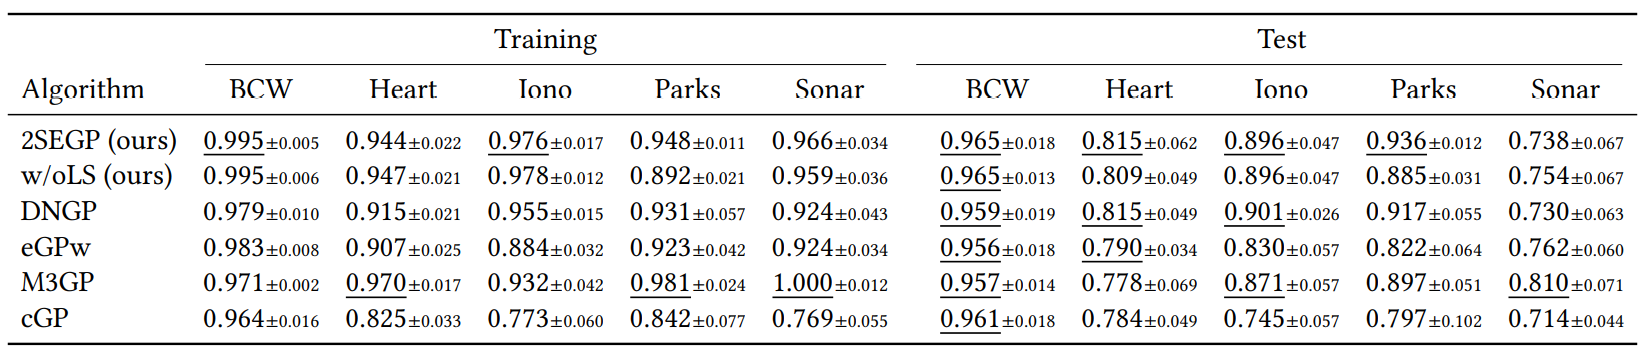
\includegraphics[scale=0.27]{Images/Classification.PNG}
	\caption{Benchmark results on the classification task, w/oLS is \textit{2SEGP} without linear scaling} \label{ClassificationImage}
\end{figure}
\begin{figure}[h]
	\centering
	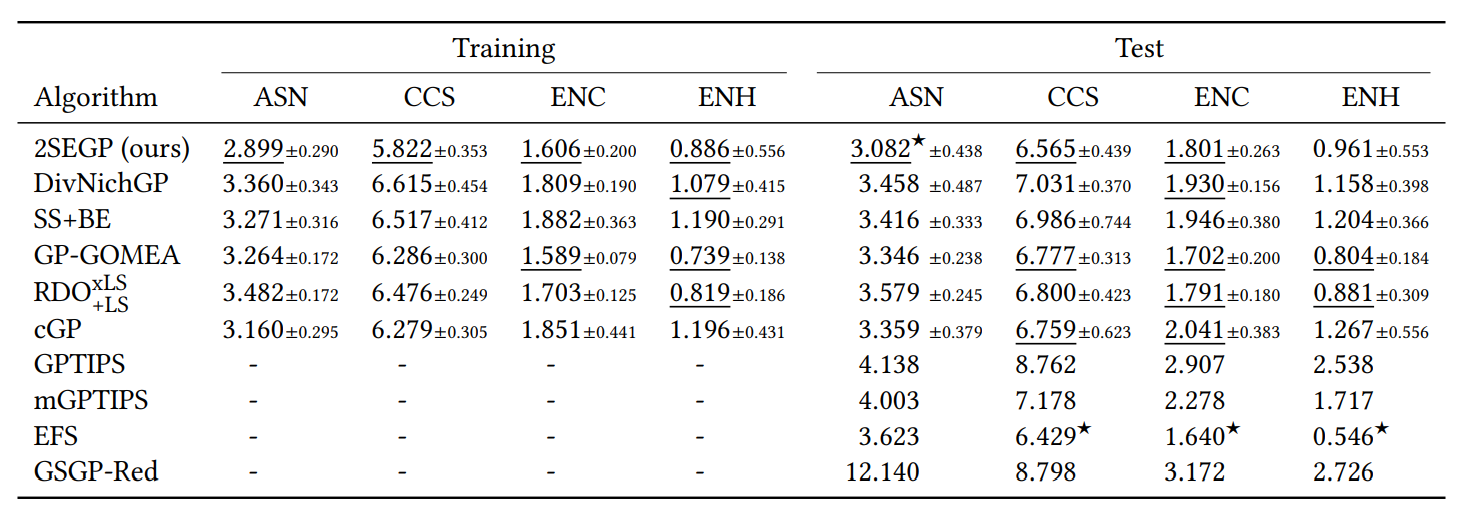
\includegraphics[scale=0.30]{Images/Regression.PNG}
	\caption{Benchmark results on the regression task} \label{RegressionImage}
\end{figure}
The results show that \textit{bagging} helps with increasing the accuracy of \textit{2SEGP} so much, that is just as good as most of the 
state-of-art algorithms, even outperforming them on a lot of tasks.

\section{Conclusion}
\label{sectionConclustion}
Combining \textit{bagging} with \textit{GP} does have major benefits in accuracy, which makes it better than pure \textit{GP}.
The only downside of this combination is the increase in computational complexity since each sample created by \textit{bagging}
will increase the time needed. The algorithm \textit{2SEGP} presented in this paper shows that only a few minor modifications 
are enough to reduce this increase in runtime, while still keeping the major benefits of the accuracy gained from \textit{bagging}. 

%
% ---- Bibliography ----
%
% BibTeX users should specify bibliography style 'splncs04'.
% References will then be sorted and formatted in the correct style.
%
\bibliographystyle{splncs04}
\bibliography{literature}
%
\end{document}
